\documentclass{article}
%\documentclass[journal]{IEEEtran}
%\documentclass{report}
%\documentclass{ActaOulu}

\usepackage{graphicx}
\usepackage{amsmath, amsthm, amssymb}
\usepackage{tensor}
\usepackage{vector}

\numberwithin{equation}{section}

% Formula Commands
\newcommand{\BtoW}{
\tensor[^B]{\left[R\right]}{^W}
}
\newcommand{\BtoWMatFull}{
  \left[ \begin{array}{ccc}
      \cos{\psi}\cos{\theta} - \sin{\phi}\sin{\psi}\sin{\theta} & \cos{\theta}\sin{\psi}+\cos{\psi}\sin{\phi}\sin{\theta} & -\cos{\phi}\sin{\theta} \\
      -\cos{\phi}\sin{\psi} & \cos{\phi}\cos{\psi} & \sin{\phi} \\
      \cos{\psi}\sin{\theta}+\cos{\theta}\sin{\phi}\sin{\psi} & \sin{\psi}\sin{\theta} - \cos{\psi}\cos{\theta}\sin{\phi} & \cos{\phi}\cos{\theta} \end{array} \right]
 }

\newcommand{\massTensor}{
  \left[ \begin{array}{ccc}
  m & 0 & 0 \\
  0 & m & 0 \\
  0 & 0 & m \end{array} \right]
}

\newcommand{\inertialTensor}{
\left[ \begin{array}{ccc}
I_{xx} & I_{xy} & I_{xz}\\
I_{yx} & I_{yy} & I_{yz} \\
I_{zx} & I_{zy} & I_{zz} \end{array} \right]
}

\newcommand{\omegaVec}{
\left[ \begin{array}{ccc}
p\\
q\\
r \end{array} \right]
}

\newcommand{\posVec}{
\left[ \begin{array}{ccc}
x\\
y\\
z \end{array} \right]
}

\newcommand{\worldCoords}{$\hat{e}_{x}, \hat{e}_{y}, \hat{e}_{z}$}
\newcommand{\bodyCoords}{$\hat{e}_{bx}, \hat{e}_{by}, \hat{e}_{bz}$}

\begin{document}

\title{Summary of Progress on the Storque 3D state space model}
\author{Ian O'Hara}

\maketitle

\begin{abstract}
A comprehensive summary on progress to date on the Storque 3D state space simulation include control.  This work is largely based on the work by \emph{Mellinger, et. al.}.
\end{abstract}

\section{Nomenclature, Coordinate Systems, and General Setup}

We'll use a Z-X-Y Euler angle setup.  $\phi$ is on $X'$, $\theta$ is on $Y''$, $\psi$ is on Z.  Note that these $X, Y, Z$ are in the body frame which is described by the unit vectors \bodyCoords, respectively.  The world frame is described by \worldCoords, and the rotation matrix from the body frame to the world frame is:
\begin{equation}
   \label{BtoWDef}
  \BtoW = \BtoWMatFull
\end{equation}
\begin{equation}
\label{massTensDef}
  \bar{\bar{M}} = \massTensor
\end{equation}
\begin{equation}
  \label{inertialTensDef}
  \bar{\bar{I}} = \inertialTensor
\end{equation}
\begin{equation}
  \label{positionDef}
  \vec{r} = \posVec
\end{equation}
\begin{equation}
\label{omegaDef}
  \vec{\omega} = \omegaVec
\end{equation}
Where $p,q,r$ are angular velocities in the body frame corresponding to the \bodyCoords  axes, respectively.
\begin{equation}
  \label{thrustAndOmegaDef}
  \left(T_1,T_2,T_3,T_4\right) and \left(\omega_1,\omega_2,\omega_3,\omega_4\right) and \left(M_1, M_2, M_3, M_4\right)
\end{equation}
Are the thrust, angular speed, and moment in the $e_{bz}$ direction of each prop (labelled in \ref{coordSys})
\begin{figure}
  \centering
  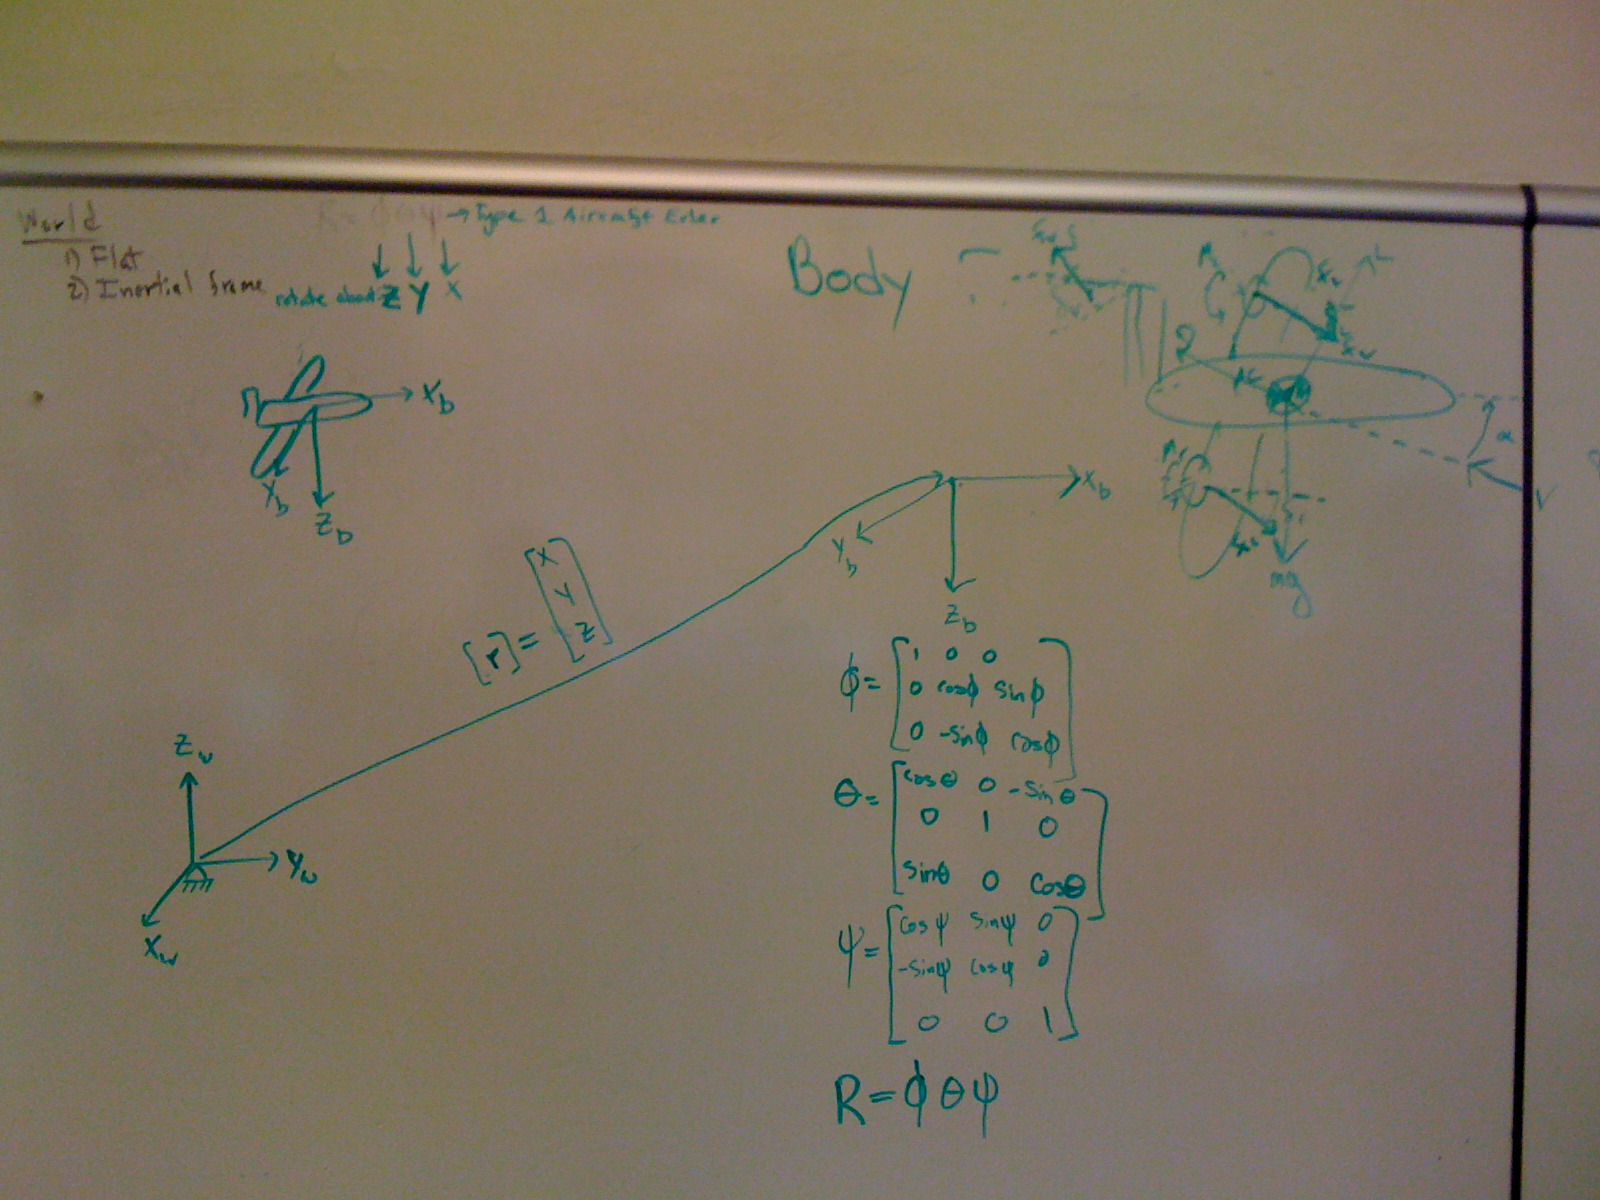
\includegraphics[width=4in]{coordSys.JPG}
  \caption{Storque coordinate system}
  \label{coordSys}
\end{figure}

\section{Equations of Motion}

\subsection{Linear Acceleration}

\begin{equation}
  \label{linAccel}
  \bar{\bar{M}} \left[ \begin{array}{ccc} 
           \ddot{x} \\ 
           \ddot{y} \\ 
           \ddot{z} \end{array} \right] 
           =
   \left[ \begin{array}{ccc}
          0 \\
          0 \\
          mg \end{array} \right]
          +
    \BtoW \left[\begin{array}{ccc}
         0 \\
         0 \\
         -T_1 - T_2 - T_3 - T_4
         \end{array}\right]
\end{equation}

\subsection{Angular Acceleration}
\begin{equation}
  \label{angAccel}
  \bar{\bar{I}} \left[ \begin{array}{ccc} \dot{p} \\ 
  							\dot{q} \\ 
							\dot{r} \end{array} \right]
  =
  \left[ \begin{array}{ccc} L\left(T_4 - T_3\right) \\ 
  				      L\left(T_1 - T_2\right) \\ 
				      M_1 + M_2 - M_3 - M_4 \end{array} \right]
				      -
				      \omegaVec \times \bar{\bar{I}} \omegaVec
\end{equation}
  
Where:

\begin{equation}
    \label{omegaDot}
    \left[ \begin{array}{ccc} \dot{p} \\ 
  					\dot{q} \\ 
					\dot{r} \end{array} \right]
					=
					nasty vector I need to look up again
\end{equation}

\section{Analysis}
\subsection{Motor Characteristics}
It has been shown by \emph{Mellinger, et. al.} and suggested by our faculty advisor Dr. Bruce D. Kothmann that the thrust and moment generated by a prop is proportional to angular velocity squared, or $T_i = K_{ti} \omega_i^2$ and $M_i = K_{mi} \omega_i^2$ where $K_{ti}$ and $K_{mi}$ are experimentally determined gains.

\emph{Mellinger, et. al.} and Dr. Kothmann also suggested that:
\[\dot{\omega_i} = K_{mot}\left(\omega_{i,com} - \omega_i\right)\]

\subsection{Equations of Motion with Motor Characteristics}
\subsubsection{Linear Acceleration}
\begin{equation}
    \label{linAccelMot}
     \bar{\bar{M}} \left[ \begin{array}{ccc} 
           \ddot{x} \\ 
           \ddot{y} \\ 
           \ddot{z} \end{array} \right] 
           =
   \left[ \begin{array}{ccc}
          0 \\
          0 \\
          mg \end{array} \right]
          +
    \BtoW \left[\begin{array}{ccc}
         0 \\
         0 \\
         K_t\left(\omega_1^2 + \omega_2^2 + \omega_3^2 + \omega_4^2\right)
         \end{array}\right]
\end{equation}

\subsubsection{Angular Acceleration}
\begin{equation}
  \label{angAccelMot}
  \bar{\bar{I}} \left[ \begin{array}{ccc} \dot{p} \\ 
  							\dot{q} \\ 
							\dot{r} \end{array} \right]
  =
  \left[ \begin{array}{ccc} K_{t}L\left(\omega_4^2 - \omega_3^2\right) \\ 
  				      K_{t}L\left(\omega_1^2 - \omega_2^2\right) \\ 
				      K_{m}\left(\omega_1^2 + \omega_2^2\right) - K_{m}\left(\omega_3^2 +\omega_4^2\right) \end{array} \right]
				      -
				      \omegaVec \times \bar{\bar{I}} \omegaVec
  \end{equation}
 Where we assume $K_{t1} = K_{t2} = ... = K_{t}$ and $K_{m1} = K_{m2} = ... = K_{m}$ because all four motor/prop combinations are identical.

\subsection{Hover Trim}
  At hover, $\dot{\vec{\omega}} = \vec{\omega} = \vec{0}$ and $\phi = \theta = \psi = 0$ and $\ddot{r}     = \dot{r} = \vec{0}$.  This says:
  \[\BtoW = \left[I\right]_{3x3} = identity\]
  And so: 
  \begin{equation}
   \left[ \begin{array}{ccc}
            0 \\
            0 \\
            mg \end{array} \right]
            =
      \BtoW \left[\begin{array}{ccc}
           0 \\
           0 \\
           K_t\left(\omega_1^2 + \omega_2^2 + \omega_3^2 + \omega_4^2\right)
           \end{array}\right]
           =
           \left[\begin{array}{ccc}
           0 \\
           0 \\
           K_t\left(\omega_1^2 + \omega_2^2 + \omega_3^2 + \omega_4^2\right)
           \end{array}\right]
 \end{equation}
  Also:
  \begin{equation}
      \left[ \begin{array}{ccc} \dot{p} \\ 
    							\dot{q} \\ 
  							\dot{r} \end{array} \right]
  				        =
      \left[ \begin{array}{ccc} 0 \\ 
    				        0 \\ 
  				        0 \end{array} \right]
  				        =
   \left[ \begin{array}{ccc} K_{t}L\left(\omega_4^2 - \omega_3^2\right) \\ 
    				      K_{t}L\left(\omega_1^2 - \omega_2^2\right) \\ 
  				      K_{m}\left(\omega_1^2 + \omega_2^2\right) - K_{m}\left(\omega_3^2 +  \omega_4^2\right) \end{array} \right]
  \end{equation}
  Which implies:
  \[\omega_1^2 = \omega_2^2 = \omega_3^2 = \omega_4^2 = \omega_{trim}^2\]
  Finally we have:
  \[4K_t\omega_{trim}^2 = mg\]
  Or:
  \begin{equation}
  \label{trimOmega} 
  \omega_{trim} = \sqrt{\frac{mg}{4K_t}}
  \end{equation}

  \subsection{Control}
  
  \subsection{Non-Linear State Space Representation}
    Our state vector is defined as:
    \begin{equation}
      \label{stateVecEqn}
      \vec{x} = \left( \begin{array}{cccccccccccccccc}x&y&z& \dot{x}& \dot{y}& \dot{z}& \phi& \theta&
       \psi& p &w &r&\omega_1&\omega_2&\omega_3&\omega_4\end{array} \right)^T
    \end{equation}
    Our input vector is:
    \begin{equation}
      \label{inputVecEqn}
      \vec{u} = \left(something\right)
    \end{equation}
    
    The rate of change of state without control is defined, in pieces, below:
    \begin{equation}
    \label{linAccelStateStep}
    \left[\begin{array}{c} \ddot{x} \\
    				   \ddot{y} \\
				   \ddot{z} \end{array} \right]
				   =
				   \left(\bar{\bar{M}}\right)^{-1}\left\{\left[ \begin{array}{ccc}
          0 \\
          0 \\
          mg \end{array} \right]
          +
    \BtoW \left[\begin{array}{ccc}
         0 \\
         0 \\
         K_t\left(\omega_1^2 + \omega_2^2 + \omega_3^2 + \omega_4^2\right)
         \end{array}\right]
\right\}
\end{equation}

\begin{equation}
\label{angAccelStateStep}
\left[\begin{array}{c}\dot{p}\\
			       \dot{q}\\
			       \dot{r} \\ \end{array} \right]
			       =
 	 \left(\bar{\bar{I}}\right)^{-1}\left\{
	  \left[ \begin{array}{ccc} K_{t}L\left(\omega_4^2 - \omega_3^2\right) \\ 
  				      K_{t}L\left(\omega_1^2 - \omega_2^2\right) \\ 
				      K_{m}\left(\omega_1^2 + \omega_2^2\right) - K_{m}\left(\omega_3^2 +\omega_4^2\right) \end{array} \right]
				      -
				      \omegaVec \times \bar{\bar{I}} \omegaVec \right\}
\end{equation}
\begin{equation}
\label{eulerDotStateStep}
\left[\begin{array}{c}\dot{\phi}\\
				\dot{\theta} \\
				\dot{\psi} \end{array} \right]
				=
		\left[ \begin{array}{ccc} \cos{\theta} & 0 & -\cos{\phi}\sin{\theta} \\
						     0 & 1 & \sin{\phi} \\
						     \sin{\theta} & 0 & \cos{\phi}\cos{\theta} \end{array} \right]^{-1}
		\left[\begin{array}{c}p\\
			       q\\
			       r \\ \end{array} \right]
\end{equation}
\begin{equation}
\label{omegaDotStateStep}
\left[\begin{array}{c} \dot{\omega_1} \\
				\dot{\omega_2} \\
				\dot{\omega_3} \\
				\dot{\omega_4} \end{array} \right]
				=
	K_{mot}\left[\begin{array}{c} \omega_{1,des} - \omega_1 \\
						   \omega_{2,des} - \omega_2 \\
						   \omega_{3,des} - \omega_3 \\
						   \omega_{4,des} - \omega_4 \end{array} \right]
\end{equation}
Where we have not defined $\omega_{i,des}$ yet.

\subsection{Linearization}
If we assume $\bar{\bar{I}}_{ij} \ll \bar{\bar{I}}_{ii}$ because of the symmetry of our design, then the $\vec{\omega} \times \bar{\bar{I}}\vec{\omega} $ term in \eqref{angAccelStateStep} is $\approx \vec{0}$.  

  \section{Conclusion}


\end{document}
